\documentclass[11pt, a4paper]{article}
\usepackage{multirow}
%\usepackage{minted}
\usepackage[slantfont,boldfont]{xeCJK}
\setCJKmainfont{SimSun}
\usepackage{indentfirst}
\usepackage{float}
\setlength{\parindent}{2em}
\setCJKmonofont{SimHei}
\input zhwinfonts
\renewcommand\figurename{图}
\renewcommand\tablename{表}

\begin{document}
\title{\bf 论文\\《UpBit: Scalable In-Memory Updatable Bitmap Indexing》\\概述}
  \author{计算机科学与技术学院\\马玉坤\\1150310618}
  \date{2017年5月9日}
  \maketitle

  \section{前言}
  该论文提出了Upbit——一种支持对数据进行高速修改或查询的位图索引的实现方法。

  \subsection{位图索引}
  位图索引(Bitmap Index)由P’ONeil在1987年提出,并在一个商用数据库系统Model 204上首次应用。在数据库中,无论是用于科研用途,还是商业用途,位图向量都被广泛应用。\cite{art3}最原始的位图索引利用位向量(Bit Vector)来表示某种被索引的属性在数据集中的索引情况。例如在表\ref{tb:table}中:在“数学成绩”一列中“优秀”这个属性的位图向量为101,分别代表小A拥有此属性、小B未拥有此属性,小C拥有此属性。将不同属性的位向量进行位逻辑运算,即可以回答各种复杂的信息。

  \begin{table}[]
    \centering
    \label{tb:table} \caption{一个普通的表}
    \begin{tabular}{|l|l|l|}
      \hline
      姓名 & 数学成绩 & 语文成绩 \\ \hline
      小A & 优秀   & 及格   \\ \hline
      小B & 良好   & 优秀   \\ \hline
      小C & 优秀   & 不及格 \\ \hline
    \end{tabular}
  \end{table}

  位图索引尽管是被设计来高效地进行大量的数据库查询操作,但相对少量的数据库修改操作有时也是必要的。如何高效的能够让位图索引在能够进行高效查询的同时进行高效的修改,是数据库领域的热门问题。

  该论文使用了维护更新向量和分块指针的方法,较好地解决了使用位图向量高效进行查询和修改操作的问题。

  \section{论文思想}

  \subsection{Update Conscious Bitvector}

  在本论文前,已有一种叫做Update Conscious Bitvector(下简称UCB)的支持修改的位图索引技术被提出。该篇论文提出的Upbit即是在UCB的基础上加以改进的成果。UCB的主要思想如下:


  使用WAH\cite{art5}算法对位向量进行压缩后,压缩后的位向量上原地修改的效率堪忧,但是容易发现,在压缩后位向量的最后面添加一位的速度是极快的。对于可修改的位图向量的优化,一个直接想法是,既然修改操作并不多,原地修改的效率堪忧,为什么不把修改操作转化为禁用(删除)+添加操作?这即是UCB(Update Conscious Bitmaps)的主要思想。

  \begin{figure}[H]
    \begin{center}
      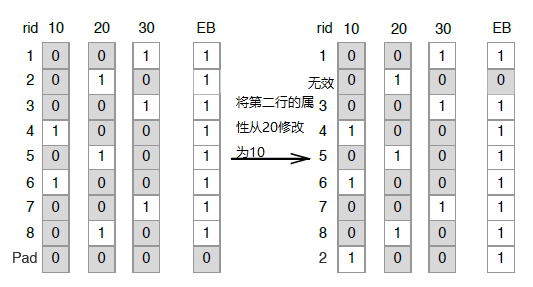
\includegraphics[width=5in]{ucb.png}
      \caption{UCB图解} \label{fig:ucb}
    \end{center}
  \end{figure}

  在UCB中,每行都有一个额外的位向量叫做存在向量(Existence Bitvector, EB)。当$EB_i$为1时,表示该行有效,否则该行无效(Invalid)。如图\ref{fig:ucb},当我们想要把第二行的值从20改为10时,我们只需要将$EB_2$设为0,然后在位向量后新建一位,并将对应的EB设为1。

  查询时,我们需要将对应的属性的位向量与存在向量进行“逻辑与”操作。

  实验中,UCB的确能极大地提高伴有少量修改操作的查询效率的提高,但是随着修改操作的积累,存在向量的复杂性将大大提高,UCB查询的效率将会极大地下降。如何使位图向量查询的效率随着修改操作积累不明显提高?这便是Upbit的创新之处。

  \subsection{Upbit}

  实际上,上一个问题的解决方案并不难。既然随着修改次数的增加,EB的复杂度提高,造成了查询的瓶颈。为什么我们不在修改次数达到一定数量级时,通过修改各个属性的位向量来维护存在向量,使存在向量保持高压缩性,提高查询效率?

  UpBit使用了这种策略。UpBit是一个新提出的位图向量方案,能够在保持修改效率较快的情况下,保持查询的效率。

  UpBit并没有只使用一个存在向量,而是对每个属性都使用了一个更新向量(Update Bitvector,UB)。每一个属性的位向量,用两个位向量经“位异或”计算得出,这两个位向量分别为值向量(Value Bitvector,VB)与更新向量(Update Bitvector,UB)。

  由于每一个属性的位向量用两个位向量经“位异或”计算得出。所以无论我们修改UB或者VB,都相当于对属性进行修改。在每次修改操作时,我们直接修改UB的值。如图\ref{fig:upbit},当我们想要把第二行的值从20修改为10,只需要把属性20对应的$UB_i$取反(从0变为1或者从1变为0),然后把属性10对应的$UB_i$取反。

  \begin{figure}[H]
    \begin{center}
      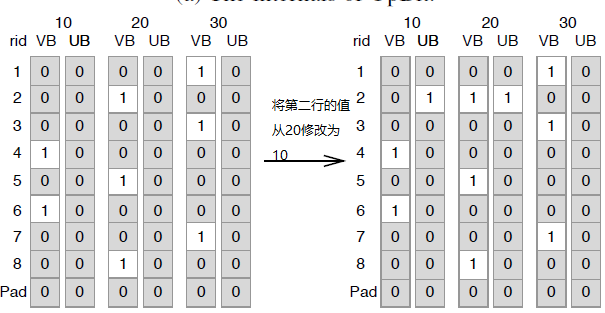
\includegraphics[width=5in]{upbit.png}
      \caption{Upbit图解}
      \label{fig:upbit}
    \end{center}
  \end{figure}


  \subsubsection{定时维护更新向量}
  当某个属性的UB的修改次数达到一定阈值时,我们将该属性的VB与UB做异或操作,将结果保存到VB中,然后将UB设为全0的向量,这便是对UB的维护。这样的维护可以保证随着修改操作积累,查询的效率仍然可以很快。

  \subsubsection{维护向量的分块指针}
  同时,UpBit还使用了第二种关键的提高效率的方法——块指针(Fence Pointers)。当我们对某一行的值进行修改时,首先就需要找到这一行修改前的值。在寻找这一行修改前的值的过程中,我们需要在每一个属性的压缩后的UB和VB中查询这一行对应的二进制位的值。如何在压缩后的位向量中,快速找到第i位的值,是一个与效率关系极大的问题。块指针的思想是:将未压缩前的位向量按下标分为若干连续的块,每一块的块大小都接近g(g是人为给定的值)。对于每个位向量,维护每一块的起始位置对应的行在压缩后的位向量中的位置,就可以在O(g+log N/g)的时间复杂度内快速在每个压缩后位向量中找到任意一行的位置,并可在O(N/g)的时间复杂度内维护修改后位向量的块指针。

  \section{基本算法}

  \subsection{获取某一行的值}

  获取第i行的值时,需要枚举值域,直到找到某个值对应的$UB$和$VB$满足$UB_i \oplus VB_i = 1$。

  \begin{figure}[H]
    \begin{center}
      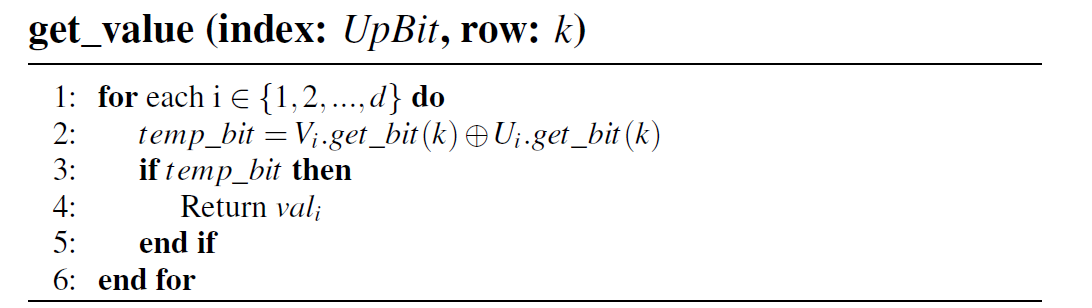
\includegraphics[width=5in]{get_value.png}
      \caption{获取某一行的值}
      \label{fig:get_value}
    \end{center}
  \end{figure}

  \subsection{更新某一行的值}

  更新某一行的值时,首先要获取当前行的原始的值(可以使用get\_value()),然后再将两个值对应的$UB_i$都分别进行取反。


  \begin{figure}[H]
    \begin{center}
      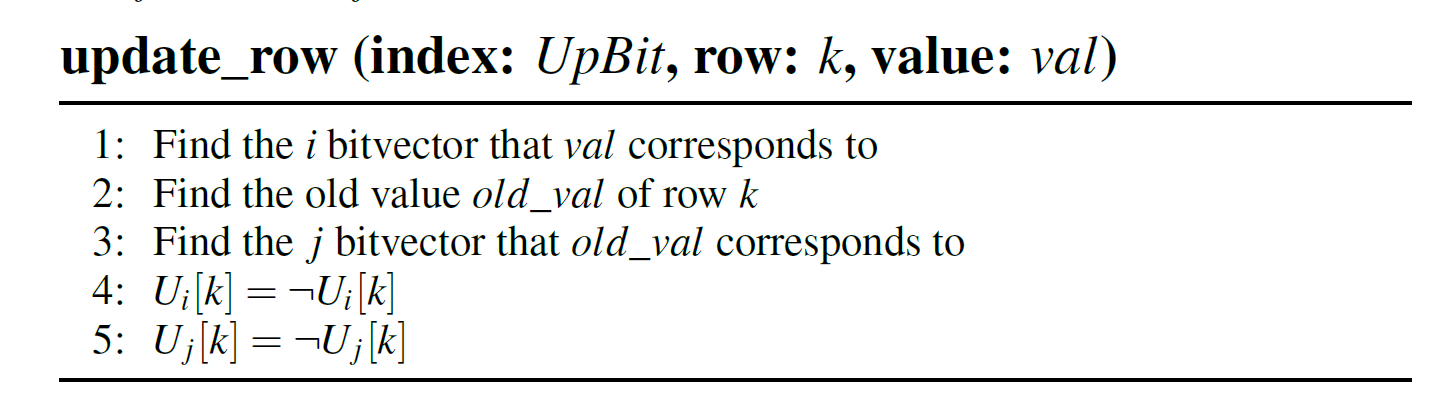
\includegraphics[width=5in]{update_row.png}
      \caption{修改某一行的值}
      \label{fig:update_row}
    \end{center}
  \end{figure}

  \subsection{合并UB与VB}

  当UB的修改次数达到一定阈值(阈值需人为设定)时,需要将UB与对应的VB合并,然后将UB置0。下图中FP为Fence Pointers。

  \begin{figure}[H]
    \begin{center}
      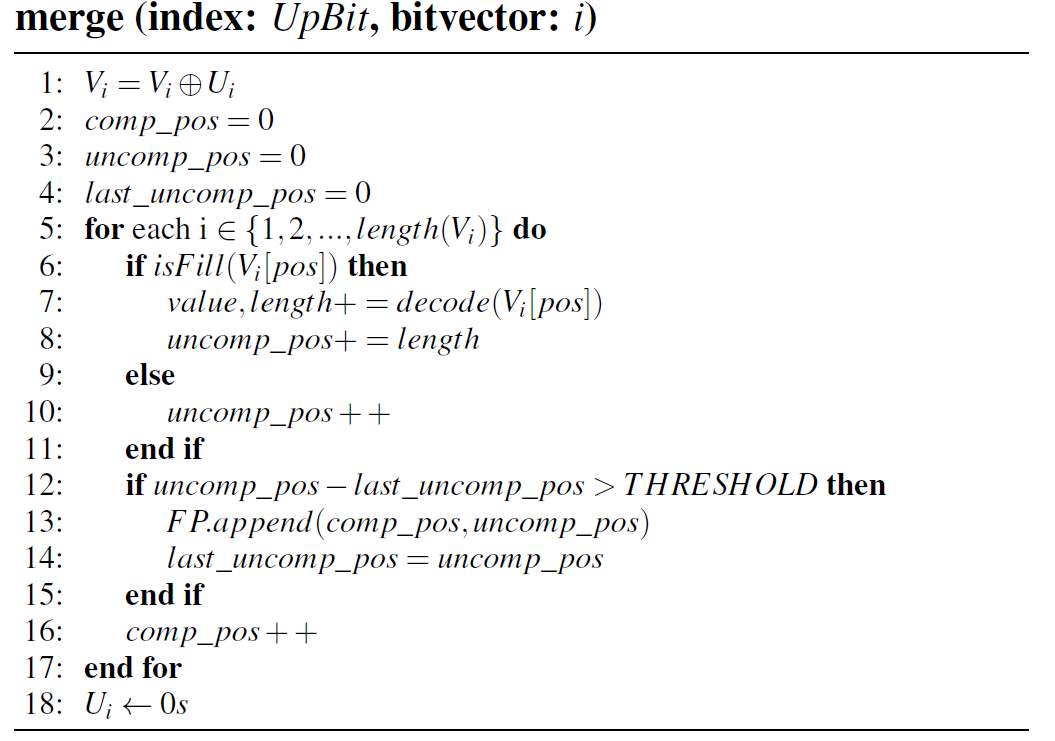
\includegraphics[width=5in]{merge.png}
      \caption{合并UB与VB}
      \label{fig:merge}
    \end{center}
  \end{figure}

  \section{算法分析}

  该算法原理巧妙简洁,并能对位图向量的效率带来极大的提升。

  \subsection{空间复杂度分析}

  由于使用了WAH压缩,其空间复杂度为$O(R)$\footnote{设行数为$R$,值域大小为$C$。}。Fence Pointers的空间复杂度与g有关,但仍小于$O(R)$。故总空间复杂度为$O(R)$。

  \subsection{时间复杂度分析}

  查询某一行的值的时间复杂度为$O(C(g + \log \frac{R}{g}))$,修改某一行的值时,由于比查询多了维护Fence Pointers的代价,故时间复杂度为$O(C(g + \log \frac{R}{g} + R/g))$。

  \subsection{举例}

  见2.2。


\renewcommand\refname{参考文献}
\begin{thebibliography}{99}
\bibitem{art1}Athanassoulis M, Yan Z, Idreos S. UpBit: Scalable In-Memory Updatable Bitmap Indexing[C]//Proceedings of the 2016 International Conference on Management of Data. ACM, 2016: 1319-1332.
\bibitem{art2}Canahuate G, Gibas M, Ferhatosmanoglu H. Update conscious bitmap indices[C]//Scientific and Statistical Database Management, 2007. SSBDM'07. 19th International Conference on. IEEE, 2007: 15-15.
\bibitem{art3}程鹏. 位图索引技术及其研究综述[J]. 科技信息, 2010 (26): 134-135.
\bibitem{art4}Wu K, Ahern S, Bethel E W, et al. FastBit: interactively searching massive data[C]//Journal of Physics: Conference Series. IOP Publishing, 2009, 180(1): 012053.
\bibitem{art5}Wu K, Otoo E J, Shoshani A. Compressing bitmap indexes for faster search operations[C]//Scientific and Statistical Database Management, 2002. Proceedings. 14th International Conference on. IEEE, 2002: 99-108.
\end{thebibliography}

\end{document}
